\documentclass[12pt]{article}

\usepackage{sbc-template}
\usepackage[utf8]{inputenc}
\usepackage[brazil,portuguese]{babel}   

\usepackage{graphicx,url}

%\usepackage[brazil]{babel}   
%\usepackage[latin1]{inputenc}  

     
\sloppy

\title{Mineração de Dados para Auxiliar na Detecção de 
\\Fraudes em Folhas de Pagamentos em Prefeituras}

\author{Janine F. Oliveira\inst{1}, Jair Bogo\inst{1}, Eriko S. Teixeira\inst{1,2}}

\address{Centro de Estudos e Sistemas Avançados do Recife (CESAR SCHOOL)\\
  AV. Cais do Apolo, 77 – Recife, PE – Brasil\\
\nextinstitute
  Universidade Federal Rural de Pernambuco (UFRPE)\\
  Recife, PE – Brasil\\
\email{jfo,jb,est@cesar.school }
}

\begin{document} 

\maketitle

\begin{abstract}
Data mining is a multidisciplinary research area, including machine learning, pattern recognition, fraud detection, data retrieval, database, statistics and more. The use of mining data applied to detect payroll fraud in government companies is a relatively new topic with several open problems. This paper presents a data mining process and an outlier technical application with a technology boxplot to demonstrate the payroll financial behavior of a Ceará state condition.
  
  \vspace{\onelineskip}
 \noindent
 \textbf{Palavras-chave}: Payroll, Public agency, Fraud Detection, Data Mining, Outlier.
\end{abstract}
     
\begin{resumo} 
 Mineração de dados é uma área de pesquisa multidisciplinar, incluindo aprendizado de máquina, reconhecimento de padrões, detecção de fraudes, recuperação de dados, banco de dados, estatísticas e outras. O uso de mineração de dados aplicado a detecção de fraudes em folha de pagamento em empresas de governo é um tema relativamente novo e com diversos problemas em abertos. Este trabalho apresenta um processo de mineração de dados e a aplicação de técnicas de outlier com a tecnologia boxplot para demonstrar o comportamento financeiro da folha de pagamento de uma prefeitura do estado do Ceará.
  
 \vspace{\onelineskip}
 \noindent
 \textbf{Keywords}: Folha de Pagamento, Órgão Público, Detecção de Fraudes, Mineração de Dados, Outlier.
\end{resumo}

\section{Introdução}
%CONTEXTUALIZAÇÃO - Prefeitura, faudes, folha de pagamento, mineração de dados
A detecção de fraudes através da análise de dados, sejam dados privados ou envolvendo dados governamentais, apresentam uma série de dificuldades e obstáculos, sendo um desafio para auditores como demostrado em \cite{ELECHI-2019}. Segundo Rockness fraude não é um problema recente e tampouco de fácil conceituação devido à existência de diversos fatores inter-relacionados, envolvendo aspectos éticos, legais, institucionais, econômicos e valores morais de determinada sociedade \cite{ROCKNESS-2005}. Ressaltam, ainda a dificuldade em diminuir ou combater fraudes, evidenciando que apenas sistemas de armazenamento de dados não são mais suficientes, sendo preciso algo que auxilie a área fiscal a analisar os dados para identificar comportamento anômalos.

%DESTACAR PROBLEMA
A \textit{Association of Certified Fraud Examiners} afirma que 27\% das empresas possui problemas na folha de pagamento, com fraude de horas extras inexistentes dos funcionários \cite{ACFE-2012}. A pesquisa realizada revela ainda que a fraude pode comprometer 5\% da receita bruta anual dessas empresas. Em empresas de governo a situação se assemelha. Segundo um estudo realizado pelo Departamento de Competitividade e Tecnologia(Decomtec) da FIESP em 2008 o custo médio anual da corrupção no Brasil representou de 1,38\% a 2,30\% do PIB, ou seja, aproximadamente R\$ 41,5 bilhões a R\$ 69,1 bilhões \cite{FIESP-2010}. Esse dinheiro público foi utilizado indevidamente por pessoas ou empresas que tomaram proveito de falhas e da falta de uma fiscalização eficaz nos gastos financeiros.

%OBJETIVO
A ciência de dados é uma das áreas da computação em maior desenvolvimento na atualidade, sendo estudada e aplicada em diversos ramos. Dhar relata que as aplicações mais relevantes da ciência de dados são os estudos relacionados a: prever eventos futuros, analisar comportamentos em massa, categorizar os mais diversos assuntos e possíveis ações a fim de trazer maior competitividade às empresas que utilizam essas técnicas \cite{DHAR-VASANT2013}. Portanto, o objetivo deste trabalho é apresentar o processo de mineração de dados que visa otimizar a fiscalização da folha de pagamento, contribuindo para redução dos erros nos repasses  dos colaboradores das prefeituras e ampliando eficacia da utilização dos recursos públicos.

%METODOLOGIA E JUSTIFICATIVA
A fim de lidar com grandes volumes de dados e auxiliar a análise de dados para prever ou minimizar fraudes na folha de pagamento, a utilização de técnicas de mineração de dados tem se mostrado de grande valia. Segundo Witten e Fank, \textit{Data Science} auxilia na obtenção de informações e também no processo de descoberta de novos conhecimentos \cite{WITTEN-FRANK2011}.


\section{Materiais e Métodos} \label{sec:firstpage}
Geralmente as prefeituras possuem um órgão responsável pelo planejamento e orçamento, na qual o mesmo é responsável por manter diversos dados e gerar todos os pagamentos mensais dos servidores, terceirizados, fornecedores entre outros na folha de pagamento, parte desses dados são aberto outros não. O conceito de dados aberto é quando qualquer pessoa pode livremente acessá-los, utilizá-los, modificá-los e compartilhá-los para qualquer finalidade \cite{OPENKNOW-2017}. Segundo dados aberto de Fortaleza, existem em média 52.080 pessoas ativas na folha de pagamento. Logo, os dados de pagamento de todas essas pessoas são fiscalizados mensalmente apenas por setores financeiros dentro de cada órgão, por alguns analistas financeiros.

Para a realização deste trabalho foi escolhida uma prefeitura do Estado do Ceará e dentro dessa prefeitura foi selecionado aleatoriamente um órgão, sendo que existiam no momento da seleção quarenta e um órgãos existentes. Visto que o regimento de pagamento pode alterar de acordo com cada categoria, cargo, nível e outras variáveis, foi optado trabalhar apenas com funcionários de um mesmo cargo que pertencem ao órgão selecionado. Logo, o público analisado neste trabalho foram de 436 pessoas ativas na folha de pagamento nos meses de: janeiro, fevereiro e março de 2019. Esses dados foram obtidos através de uma base com mais de 228 gigas de dados, relacionados a folha de pagamento, contendo 679 tabelas em um banco de dados da Oracle. Para ter acesso a essas bases de dados foi assinado um termo de confidencialidade e sigilo, no qual os envolvidos na pesquisa se comprometem a utiliza-las apenas para fins acadêmicos e a não usufruir as informações confidenciais, para gerar benefícios financeiros próprio exclusivo e/ou unilateral, presente ou futuro, ou para o uso de terceiros.

\section{Abordagem Proposta e Resultados Obtidos}
Na figura \ref{fig:Processo} é ilustrado o diagrama esquemático do funcionamento da abordagem proposta para o processo de mineração de dados em uma folha de pagamento. Os bancos de dados analisados possuem dados financeiros de 2004 até 2019, portanto existem muitas tabelas e muitas colunas. Então inicialmente foram analisados todos esses dados disponíveis, com isso pode-se selecionar aproximadamente 80 tipos de dados diferentes e que possuem mais relevância para o salário de um funcionário, como por exemplo quantidade de horas extras, números de dependentes, escolaridade entre outros. A próxima etapa foi idealizar um modelo com todos esses dados brutos, como por exemplo quantidade de dependentes, idade, sexo, horas extras etc. Em seguida foi utilizado uma ferramenta \textit{open source} de \textit{Extract Transform Load} (ETL) para tratamento, exploração de novas variáveis e carregamento de dados para o modelo, gerando assim os dados processados. Na fase de mineração de dados analisamos possíveis padrões de comportamentos do grupo selecionado e apresentamos os resultados aos analistas fiscais que validam segundo a legislação se é ou não problema de fraude. Caso não seja fraude o processo inicia-se novamente para verificar outro modelos ou outros dados para continuar o processo de fiscalização. Porém caso seja validado que foi uma fraude gera um conhecimento do caso e solicitação de correções nos sistemas financeiros para que não ocorrer o erro novamente na folha de pagamento. 

\begin{figure}[!ht]
    \centering
    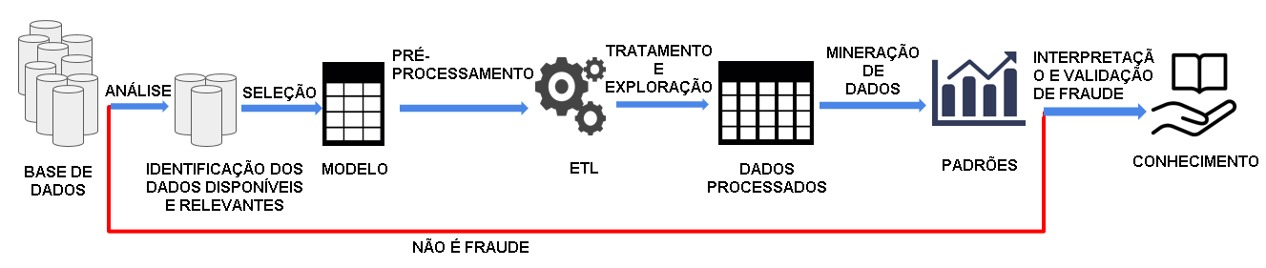
\includegraphics[width=.9\textwidth]{Processo2.png}
    \caption{Processo Mapeado para Mineração de Dados.}
    \label{fig:Processo}
\end{figure}

Na fase de analisar os dados, após as transformações, foi possível identifica valores atípicos contidos na base de dados, que podemos chamar de ruídos ou \textit{outlier}. Um \textit{outlier} é uma observação discrepante dentro do conjunto de dados, contendo um valor maior ou menor do que a maioria dos outros dados. Segundo Ping, a descoberta de valores atípicos evidencia um comportamento inesperado no conjunto de dados, devido à variabilidade na medição ou por indicar erro experimental \cite{PING2010}. Na figura \ref{fig:Outlier} é ilustrado um \textit{outlier} relacionado a valores salariais, usando a técnica \textit{boxplot}, podemos observar que existem muitos pontos acima da média e alguns abaixo. 

\begin{figure}[!ht]
    \centering
    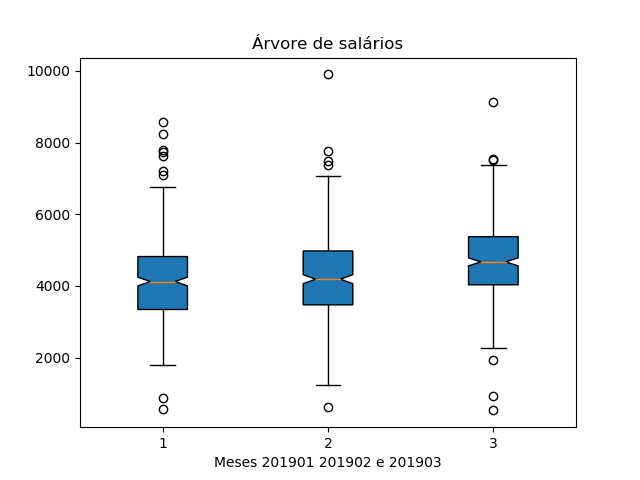
\includegraphics[width=.6\textwidth]{Outlier.png}
    \caption{Boxplot da base de dados da prefeitura com dados salariais.}
    \label{fig:Outlier}
\end{figure}

Pode-se observar ainda na figura \ref{fig:Outlier} que a média salarial do grupo estudado está entre 5 a 3 mil reais, porém existem duas pessoas que estão ganhando quase o dobro da média salarial. Após chegar esses resultados cabe aos analistas fiscais analisarem as anomalias identificadas após a mineração e verificar se existe ou não fraudes de acordo com a legislação.

\section{Considerações Finais}

%TRABALHOS FUTUROS
O principal objetivo deste trabalho foi mapear um processo de mineração de dados e apresentar um \textit{outlier} com relevância gerado a partir desse processo com dados minerado de uma folha de pagamento. Em trabalhos futuros pretende-se dar continuidade na pesquisa aplicando técnicas de \textit{Machine Learning} e criar um algoritmo que gere índices de prioridades dos dados suspeitos para auxiliar os analistas financeiros a priorizar os casos mais graves. Além disso, almeja-se ampliar o público do estudo para todos os funcionário de uma prefeitura, fazendo com que o modelo categorize os funcionário na mesma categoria (perfil) e aplique os algoritmos para auxiliar na detecção de comportamentos anômalos.

\bibliographystyle{sbc}
\bibliography{sbc-template}

\end{document}
